\documentclass{article}
\usepackage{amsmath, amssymb, hyperref}
\usepackage{graphicx}
\usepackage {mathpartir}


% Double brackets
\newcommand{\ldb}{[\![}
\newcommand{\rdb}{]\!]}
\newcommand{\ldrb}{(\!(}
\newcommand{\rdrb}{)\!)}
\newcommand{\lrbb}{(\!|}
\newcommand{\rrbb}{|\!)}
\newcommand{\lliftb}{\langle\!|}
\newcommand{\rliftb}{|\!\rangle}
%\newcommand{\plogp}{:\!-}
\newcommand{\plogp}{\leftarrow}
%\newcommand{\plogp}{\coloneq}
% \newcommand{\lpquote}{\langle}
% \newcommand{\rpquote}{\rangle}
% \newcommand{\lpquote}{\lceil}
% \newcommand{\rpquote}{\rceil}
\newcommand{\lpquote}{\ulcorner}
\newcommand{\rpquote}{\urcorner}
\newcommand{\newkw}{\nu}
\newcommand{\dblhdlarrow}{\texttt{<\!<\!-}}
\newcommand{\dbltllarrow}{\texttt{<\!=}}
\newcommand{\sngllarrow}{\texttt{<\!-}}
\newcommand{\dblhdlrarrow}{\texttt{<\!<\!-\!>\!>}}
\newcommand{\dbltllrarrow}{\texttt{<\!=\!>}}
\newcommand{\sngllrarrow}{\texttt{<\!-\!>}}

% SYNTAX
\newcommand{\id}[1]{\texttt{#1}}
\newcommand{\none}{\emptyset}
\newcommand{\eps}{\epsilon}
\newcommand{\set}[1]{\{#1\}}
\newcommand{\rep}[2]{\id{\{$#1$,$#2$\}}}
\newcommand{\elt}[2]{\id{$#1$[$#2$]}}
\newcommand{\infinity}{$\infty$}

\newcommand{\pzero}{\mathsf{0}}
\newcommand{\seq}{\mathsf{\id{,}}}
\newcommand{\all}{\mathsf{\id{\&}}}
\newcommand{\choice}{\mathsf{\id{|}}}
\newcommand{\altern}{\mathsf{\id{+}}}
\newcommand{\juxtap}{\mathsf{\id{|}}}
\newcommand{\concat}{\mathsf{.}}
\newcommand{\punify}{\mathsf{\id{:=:}}}
\newcommand{\fuse}{\mathsf{\id{=}}}
\newcommand{\scong}{\mathsf{\equiv}}
\newcommand{\nameeq}{\mathsf{\equiv_N}}
\newcommand{\alphaeq}{\mathsf{\equiv_{\alpha}}}
\newcommand{\arrvec}[1]{\overrightarrow{#1}}
\newcommand{\names}[1]{\mathsf{N}(#1)}
\newcommand{\freenames}[1]{\mathsf{FN}(#1)}
\newcommand{\boundnames}[1]{\mathsf{BN}(#1)}
%\newcommand{\lift}[2]{\texttt{lift} \; #1 \concat #2}
\newcommand{\binpar}[2]{#1 \mathsf{|} #2}
\newcommand{\outputp}[2]{#1\mathsf{!}(#2)}
\newcommand{\prefix}[3]{\mathsf{for(}#2 \leftarrow #1 \mathsf{)} #3}
%%\newcommand{\lift}[2]{#1 \lliftb #2 \rliftb}
\newcommand{\lift}[2]{#1 \mathsf{!}(#2)}
\newcommand{\clift}[1]{\lliftb #1 \rliftb}
\newcommand{\quotep}[1]{\mathsf{@} #1}
\newcommand{\dropn}[1]{\mathsf{*} #1}
\newcommand{\procn}[1]{\stackrel{\cdot}{#1}}
\newcommand{\spacen}[2]{\mathsf{@}\langle #1, #2 \rangle}

\newcommand{\newp}[2]{(\newkw \; #1 ) #2}
\newcommand{\bangp}[1]{! #1}

\newcommand{\substp}[2]{\{ \quotep{#1} / \quotep{#2} \}}
\newcommand{\substn}[2]{\{ #1 / #2 \}}

\newcommand{\psubstp}[2]{\widehat{\substp{#1}{#2}}}
\newcommand{\psubstn}[2]{\widehat{\substn{#1}{#2}}}

\newcommand{\applyp}[2]{#1 \langle #2 \rangle}
\newcommand{\absp}[2]{( #1 ) #2}
\newcommand{\annihilate}[1]{#1^{\times}}
\newcommand{\dualize}[1]{#1^{\bullet}}
\newcommand{\ketp}[1]{\mathsf{|}#1 \rangle}
\newcommand{\brap}[1]{\langle #1 \mathsf{|}}
\newcommand{\testp}[2]{\langle #1 \mathsf{|} #2 \rangle}
\newcommand{\testnp}[3]{\langle #1 \mathsf{|} #2 \mathsf{|} #3 \rangle}

\newcommand{\transitions}[3]{\mathbin{#1 \stackrel{#2}{\longrightarrow} #3}}
\newcommand{\meaningof}[1]{\ldb #1 \rdb}
\newcommand{\pmeaningof}[1]{\ldb #1 \rdb}
\newcommand{\nmeaningof}[1]{\lrbb #1 \rrbb}

\newcommand{\Proc}{\mathsf{Proc}}
\newcommand{\QProc}{\quotep{\mathsf{Proc}}}
\newcommand{\MixSumProc}{\mathsf{MixSumProc}}

\newcommand{\entailm}{\mathbin{\vdash_{\mathfrak m}}} %matching
\newcommand{\entailp}{\mathbin{\vdash_{\mathfrak p}}} %behavioral
\newcommand{\entailv}{\mathbin{\vdash_{\mathfrak v}}} %validation
\newcommand{\congd}{\mathbin{\equiv_{\mathfrak d}}}
\newcommand{\congs}{\mathbin{\equiv_{\mathfrak s}}}
\newcommand{\congp}{\mathbin{\equiv_{\mathfrak p}}}
%\newcommand{\logequiv}{\mathbin{\leftrightarrow}}

\newcommand{\barb}[2]{\mathbin{#1 \downarrow_{#2}}}
\newcommand{\dbarb}[2]{\mathbin{#1 \Downarrow_{#2}}}

% From pi-duce paper
\newcommand{\red}{\rightarrow}
\newcommand{\wred}{\Rightarrow}
\newcommand{\redhat}{\hat{\longrightarrow}}
\newcommand{\lred}[1]{\stackrel{#1}{\longrightarrow}} %transitions
\newcommand{\wlred}[1]{\stackrel{#1}{\Longrightarrow}}

\newcommand{\opm}[2]{\overline{#1} [ #2 ]} % monadic
\newcommand{\ipm}[2]{{#1} ( #2 )} 
\newcommand{\ipmv}[2]{{#1} ( #2 )} % monadic
\newcommand{\parop}{\;|\;}		% parallel operator
\newcommand{\patmatch}[3]{#2 \in #3 \Rightarrow #1}
\newcommand{\sdot}{\, . \,}		% Space around '.'
\newcommand{\bang}{!\,}
%\newcommand{\fuse}[1]{\langle #1 \rangle}		
\newcommand{\fusion}[2]{#1 = #2} % fusion prefix/action
\newcommand{\rec}[2]{\mbox{\textsf{rec}} \, #1. \, #2}
\newcommand{\match}[2]{\mbox{\textsf{match}} \; #1 \; \mbox{\textsf{with}} \; #2}
\newcommand{\sep}{:}
\newcommand{\val}[2]{\mbox{\textsf{val}} \; #1 \; \mbox{\textsf{as}} \; #2}

\newcommand{\rel}[1]{\;{\mathcal #1}\;} %relation
\newcommand{\bisim}{\stackrel{.}{\sim}_b} %bisimilar
\newcommand{\wb}{\approx_b} %weak bisimilar
\newcommand{\bbisim}{\stackrel{\centerdot}{\sim}} %barbed bisimilar
\newcommand{\wbbisim}{\stackrel{\centerdot}{\approx}} %weak barbed bisimilar
\newcommand{\bxless}{\lesssim}	%expansion less (amssymb required)
\newcommand{\bxgtr}{\gtrsim}	%expansion greater (amssymb required)
\newcommand{\beq}{\sim}		%barbed congruent
\newcommand{\fwbeq}{\stackrel{\circ}{\approx}}	%weak barbed congruent
\newcommand{\wbeq}{\approx}	%weak barbed congruent
\newcommand{\sheq}{\simeq}	%symbolic hypereq
\newcommand{\wbc}{\approx_{cb}}

% rho logic

\newcommand{\ptrue}{\mathbin{true}}
\newcommand{\psatisfies}[2]{#1 \models #2}
\newcommand{\pdropf}[1]{\rpquote #1 \lpquote}
\newcommand{\plift}[2]{#1 \lliftb #2 \rliftb}
\newcommand{\pprefix}[3]{\langle #1 ? #2 \rangle #3}
\newcommand{\pgfp}[2]{\textsf{rec} \; #1 \mathbin{.} #2}
\newcommand{\pquant}[3]{\forall #1 \mathbin{:} #2 \mathbin{.} #3}
\newcommand{\pquantuntyped}[2]{\forall #1 \mathbin{.} #2}
\newcommand{\riff}{\Leftrightarrow}

\newcommand{\PFormula}{\mathbin{PForm}}
\newcommand{\QFormula}{\mathbin{QForm}}
\newcommand{\PropVar}{\mathbin{\mathcal{V}}}

% qm notation
\newcommand{\state}[1]{\juxtap #1 \rangle}
\newcommand{\event}[1]{\langle #1 \juxtap}
\newcommand{\innerprod}[2]{\langle #1 \juxtap #2 \rangle}
\newcommand{\prmatrix}[2]{\juxtap #1 \rangle \langle #2 \juxtap}
\newcommand{\fprmatrix}[3]{\juxtap #1 \rangle #2 \langle #3 \juxtap}

% End piduce contribution

\newcommand{\typedby}{\mathbin{\:\colon}}
\newcommand{\mixedgroup}[1]{\id{mixed($#1$)}}
\newcommand{\cast}[2]{\id{CAST AS} \; #1 \; (#2)}
\newcommand{\bslsh}{\mathbin{\id{\\}}}
\newcommand{\bslshslsh}{\mathbin{\id{\\\\}}}
\newcommand{\fslsh}{\mathbin{\id{/}}}
\newcommand{\fslshslsh}{\mathbin{\id{//}}}
\newcommand{\bb}[1]{\mbox{#1}}
\newcommand{\bc}{\mathbin{\mathbf{::=}}}
\newcommand{\bm}{\mathbin{\mathbf\mid}}
%\newcommand{\bm}{\mathbin{\mathbf\mid}}
\newcommand{\be}{\mathbin{=}}
\newcommand{\bd}{\mathbin{\buildrel {\rm \scriptscriptstyle def} \over \be}}
%\newcommand{\category}[1]{\mbox{\bf #1}}

\newcommand{\prefixt}[3]{\mathbf{for}\mathbf{(}\mathbf{#2} \leftarrow \mathbf{#1} \mathbf{)} \mathbf{#3}}
\newcommand{\outputt}[2]{\mathbf{#1}\mathsf{!}(\mathbf{#2})}
\newcommand{\dropt}[1]{\mathbf{*} \mathbf{#1}}
\newcommand{\quotet}[1]{\mathbf{@} \mathbf{#1}}
\newcommand{\commr}[5]{\mathsf{comm(}#1, #2, #3, #4, #5 \mathsf{)}}
\newcommand{\commt}[5]{\mathsf{comm(}#1, #2, #3, #4, $5 \mathsf{)}}
\newcommand{\binparx}[2]{\mathsf{par}(#1, #2)}
\newcommand{\binpart}[2]{\mathbf{par}(#1, #2)}
\newcommand{\binparpt}[2]{#1 \mathsf{|} #2}
\newcommand{\binpartl}[2]{\mathsf{par}_{L}(#1, #2)}
\newcommand{\binpartr}[2]{\mathsf{par}_{R}(#1, #2)}

%GRAMMAR
\newlength{\ltext}
\newlength{\lmath}
\newlength{\cmath}
\newlength{\rmath}
\newlength{\rtext}

\settowidth{\ltext}{complex type name}
\settowidth{\lmath}{$xxx$}
\settowidth{\cmath}{$::=$}
\settowidth{\rmath}{\id{attributeGroup}}
\settowidth{\rtext}{repetition of $g$ between $m$ and $n$ times}

\newenvironment{grammar}{
  \[
  \begin{array}{l@{\quad}rcl@{\quad}l}
  \hspace{\ltext} & \hspace{\lmath} & \hspace{\cmath} & \hspace{\rmath} & \hspace{\rtext} \\
}{
  \end{array}\]
}

% Over-full v-boxes on even pages are due to the \v{c} in author's name
%\vfuzz2pt % Don't report over-full v-boxes if over-edge is small

% THEOREM Environments ---------------------------------------------------
% MATH -------------------------------------------------------------------
 \newcommand{\veps}{\varepsilon}
 \newcommand{\To}{\longrightarrow}
 \newcommand{\h}{\mathcal{H}}
 \newcommand{\s}{\mathcal{S}}
 \newcommand{\A}{\mathcal{A}}
 \newcommand{\J}{\mathcal{J}}
 \newcommand{\M}{\mathcal{M}}
 \newcommand{\W}{\mathcal{W}}
 \newcommand{\X}{\mathcal{X}}
 \newcommand{\BOP}{\mathbf{B}}
 \newcommand{\BH}{\mathbf{B}(\mathcal{H})}
 \newcommand{\KH}{\mathcal{K}(\mathcal{H})}
 \newcommand{\Real}{\mathbb{R}}
 \newcommand{\Complex}{\mathbb{C}}
 \newcommand{\Field}{\mathbb{F}}
 \newcommand{\RPlus}{\Real^{+}}
 \newcommand{\Polar}{\mathcal{P}_{\s}}
 \newcommand{\Poly}{\mathcal{P}(E)}
 \newcommand{\EssD}{\mathcal{D}}
 \newcommand{\Lom}{\mathcal{L}}
 \newcommand{\States}{\mathcal{T}}
 \newcommand{\abs}[1]{\left\vert#1\right\vert}
% \newcommand{\set}[1]{\left\{#1\right\}}
%\newcommand{\seq}[1]{\left<#1\right>}
 \newcommand{\norm}[1]{\left\Vert#1\right\Vert}
 \newcommand{\essnorm}[1]{\norm{#1}_{\ess}}

%%% NAMES
\newcommand{\Names}{{\mathcal N}}
\newcommand{\Channels}{{\sf X}}
\newcommand{\Variables}{{\mathcal V}}
\newcommand{\Enames}{{\mathcal E}}
\newcommand{\Nonterminals}{{\mathcal S}}
\newcommand{\Pnames}{{\mathcal P}}
\newcommand{\Dnames}{{\mathcal D}}
\newcommand{\Types}{{\mathcal T}}

\newcommand{\fcalc}{fusion calculus}
\newcommand{\xcalc}{${\mathfrak x}$-calculus}
\newcommand{\lcalc}{$\lambda$-calculus}
\newcommand{\pic}{$\pi$-calculus}
\newcommand{\spic}{spi-calculus}
\newcommand{\rhoc}{$\rho$-calculus}
\newcommand{\rhol}{$\rho$-logic}
\newcommand{\hcalc}{highwire calculus}
\newcommand{\dcalc}{data calculus}
%XML should be all caps, not small caps. --cb
%\newcommand{\xml}{\textsc{xml}}
\newcommand{\xml}{XML} 
 

\newcommand{\mycomment}[1]{}
\newcommand{\MC}{\mathsf{MeTTaCycle}}
\newcommand{\FD}{\mathsf{F1R3Dr1v3}}
\newcommand{\FF}{\mathsf{F1R3FLY.io}}
\newcommand{\RS}{\mathsf{RSpace}}

\title{$\MC$ Architecture Proposal}
\author{}
\date{}

\begin{document}

\maketitle

\tableofcontents

\section{Introduction}

$\MC$ is the codename for a new decentralized AI platform.  The network will have agents, both human and AI, who can share digital assets of all kinds, attenuate and delegate access to those assets, and make powerful queries about each other's content.  

We anticipate at least two interface points between humans and the network; both of these will be based on existing user interfaces with which users are already familiar.  The first is through the operating system, where $\FD$ will be mounted into the filesystem.  The second will be based on existing open source social networking software, currently BlueSky and Mastodon.

$\MC$, as its name suggests, will feature a version of the MeTTa programming language.  The driving concept for MeTTa is the idea that intelligence opportunistically creates theories of computation to suit the domain in which the intelligence is operating.  $\MC$ intends to connect many theories operating in many domains, and to enable reasoning about these interactions.

\subsection{The MeTTa Kernel}

SingularityNet hopes that MeTTa will be a language in which one can describe a theory of computation and get an efficient interpreter that is suited for smart contracts on a blockchain~\cite{GoertzelMeredith2024}.

Without reproducing much of MeTTa's internals explicitly in the theory, MeTTa currently cannot model different evaluation strategies for lambda calculus, cannot model the semantics of the $\pi$ calculus and other mobile process calculi, and has several other problems preventing it from living up to this vision.  We propose an architecture based on category theoretical concepts that will enable MeTTa to:
\begin{itemize}
    \item specify the semantics of any discrete theory of computation
    \item generate an efficient interpreter for that theory
    \item generate a sound type system customized to that theory
    \item support concurrency
    \item support transactions
\end{itemize}
and more.

Section \ref{Theories of computation} attempts to express some theories of computation in MeTTa and uncovers some problems.  Section \ref{A way forward} describes graph-structured lambda theories (GSLTs), which solve the expressability problems.  Section \ref{Generating an interpreter and a type system} shows how from a GSLT we can generate an efficient interpreter and a sound type system.  The resulting compiled language is concurrent and transactional. Section \ref{Queries} returns to the need to query a fact database and examines the kinds of interesting query one can express in this system.

\subsection{Decentralization}

Were the deployment of an execution environment for MeTTa SingularityNet's only goal the $\MC$ architecture would comprise the elements above. However, SingularityNet's goals include a decentralized framework for AI, AGI, and ASI. As such, the architecture must also address a security model for deployment of execution outside of the protective womb of a firewall. Further, it must embrace integration with a number of third party services. Despite these additional constraints and their corresponding remedies, $\MC$ must also be accessible and not hidden behind arcane or cryptic command line interfaces.

To achieve the former we adopt a capabilities driven tokenization model. Access to compute and storage are mediated by (object) capabilities represented as tokens. See the \ref{Security model} for details. To achieve the latter we provide integration of $\MC$ with the file systems for the major operating systems; and, with major social media platforms. See \ref{Deployment and integration}.

Finally, to achieve decentralization the $\MC$ architecture needs to include fault-tolerance balanced against the need to replicate data everywhere. It achieves this by delivering a sharded, heterogeneous consensus mechanism. Each shard represents a unit of fault-tolerance governed by a consensus mechanism. Shards may be organized into a tree. Parent shards delegate to children when transactions only involve resources confined to a single child shard, but provide a governing consensus for transactions that implicate resources spanning sibling shards.

\section{Market requirements}

The demand for decentralized digital asset management systems is on
the rise. By digital assets we don’t merely mean “tokens” as used in
BTC or ETH. Rather, we mean digitally recorded and stored information
from medical records to code (such as is found in GitHub); and we
expand this scope to agentic services that act on the behalf of their
users. The $\MC$ architecture provides such a digital asset
management service that guarantees the security model of Byzantine
fault tolerant networks (BTC, ETH) with the throughput and scale of
crash fault tolerant networks (Google Drive, Dropbox). This makes it
dramatically more secure and useful than any of the incumbent
platforms.

While the crash fault tolerant cloud-based networks have scaled to
serve millions of concurrent active users, they have been plagued by
hacks like Snowflake, Crowdstrike, and many others. By contrast, the
Byzantine fault tolerant networks (such as BTC) have huge unclaimed
``bug bounties''. Billions of dollars of assets have been flowing
through the BTC network for almost two decades without a successful
hack that would allow such a claim to be made. Nevertheless, although
the latter networks benefit from using Byzantine fault tolerant
technology, they are in themselves unable to scale --- a significant
limitation. $\MC$ scales to match the throughput characteristics of the
crash fault tolerant networks (CFTNs) and does this while also
supplying the security of the Byzantine fault tolerant networks
(BFTNs).

Furthermore, one of the crucial features of the CFTNs is their
searchability. One of the most important features enabling the new
global economy is search. When everyone with an Internet connection
became able to search --- for jobs or employees, goods, services, news,
analysis, etc. --- the global digital market became a reality,
supplanting oil as the most valuable sector. $\MC$ brings the
searchability of the CFTNs to the BFTNs. This not only means that data
stored on $\MC$ networks can be searched. It also means it can be
fed to and integrated with emerging AI solutions. Specifically,
$\MC$’s smart contracting language is, by design, a transactional
query language that works across an entire $\MC$ network at
scale, on the one hand; and a state of the art AI language on the other.

Unlike the BFTNs where tokenization seems to be primarily to encourage
trading, the key role of tokenization in $\MC$ networks is
fractional security. A token is a key to a unit of compute or a unit
of storage. Imagine if, rather than handing over your Netflix password
to your family members, you gave them an allotment of tokens, each one
representing a prescribed number of viewing hours. That’s what
$\MC$ tokens represent: a very fine-grained security mechanism
that enables careful accounting and auditing of system use and asset
access.

Most enterprises need a scalable storage solution. Typical
implementations bolt the security and accounting models on the side
and are subject to hacks along both interfaces (security and
accounting). In $\MC$ these two have been seamlessly integrated and
baked into searchable, transactional storage.

\section{High-performance MeTTa Kernel}

\subsection{Theories of computation}
\label{Theories of computation}

In this section, we attempt to implement a couple of theories of computation in MeTTa and uncover some missing features and some problems with the current implementation.

\subsubsection{The theory of lambda calculus}
MeTTa can model the operational semantics of certain virtual machines using a pattern similar to those of platforms like K Framework~\cite{kframework}.  Here's a formalization of the lambda calculus in MeTTa, with an evaluation strategy that reduces terms everywhere except under a lambda:

\begin{verbatim}
; -- The theory of lambda calculus

(: T Sort)
(: App (-> T T T))
(: Lam (-> (-> T T) T))
(= (App (Lam $f) $v) ($f $v))   ; Beta reduction

; -- Named functions due to lack of lambda in MeTTa

(: ident (-> T T))
(= (ident $x) $x)

(: omega (-> T T))
(= (omega $x) (App $x $x))

(: Omega (-> T T))
(= (Omega $x) (App (Lam omega) (Lam omega)))

; -- Example reductions

!(App X (App (Lam ident) Y))    ; [(App X Y)]
!(Lam Omega)                    ; [(Lam Omega)]
;!(App (Lam omega) (Lam omega)) ; infinite loop
\end{verbatim}

The theory introduces \verb+T+ as a sort, essentially the generator in the grammar for terms.  It then declares the term constructors: \verb+App+ takes two terms and produces a term, while \verb+Lam+ takes a function from terms to terms and produces a term.  By using a function type, the theory can avoid modeling explicit substitution and alpha equivalence as part of the grammar by bootstrapping \verb+Lam+ using the binders in MeTTa itself.  Finally, the theory declares the beta rule.

Note that there's nothing in the theory corresponding to the rule defining the evaluation strategy:

\[ \frac{{\tt T} \leadsto {\tt T'} \quad {\tt U} \leadsto {\tt U'}}{\mbox{\tt (App T U)} \leadsto \mbox{\tt (App T' U')}}. \]

The evaluation strategy is hardcoded into the MeTTa interpreter.  We could not, for instance, choose to reduce solely in head position:

\[ \frac{{\tt T} \leadsto {\tt T'}}{\mbox{\tt (App T U)} \leadsto \mbox{\tt (App T' U)}} \]

or to reduce under a lambda without considerably more machinery.

\subsubsection{The theory of RHO calculus}

Unfortunately, MeTTa is also unable to model the RHO calculus~\cite{MeredithRadestock2005} (a Reflective Higher-Order pi calculus) in a straightforward way:

\begin{verbatim}
(: P Sort)
(: N Sort)
(: Zero P)
(: Par (-> P P P))
(: Send (-> N P P))
(: Recv (-> N (-> N P) P))
(: At (-> P N))
(: Run (-> N P))
(= (Par (Send $chan $proc) (Recv $chan $cont)) ($cont (At $proc)))
(= (At (Run $n)) $n)
(= (Run (At $p)) $p)

; -- Problem: no support for structural equivalence.
; -- RHO terms form a commutative monoid, but in MeTTa
; -- the commutativity rewrite causes an infinite loop.

; (= (Par $p1 $p2) (Par $p2 $p1)) ; commutative
(= (Par $p Zero) $p) ; unital
(= (Par ((Par $p1 $p2) $p3) (Par $p1 (Par $p2 $p3)))) ; assoc.

; -- Helpers

(: nil (-> N P))
(= (nil $n) Zero)
(: chan (-> N))
(= (chan) (At Zero))

; -- Problem: reduction under a Send.
; -- According to RHO semantics, the printed process below should
; -- not reduce, but MeTTa reduces it to (Send (At Zero) Zero).

(: Proc (-> P))
(= (Proc) (Par (Send (chan) Zero) (Recv (chan) nil)))
!(Send (chan) (Proc))
\end{verbatim}

\noindent MeTTa does well at modeling the sorts and term constructors.  There are sorts for Processes and Names of channels, five term constructors, and three rewrite rules.  But RHO calculus terms (as in all pi calculi) should be considered only up to structural congruence.  The term constructors form a commutative monoid under \verb+Par+, where \verb+Zero+ is the unit.  MeTTa has no concept of structural congruence.

One could argue that detecting whether two words are in the same equivalence class is, in general, undecidable, and any real implementation would use something like a normal form or a hash table to eliminate the detection problem.  The Rholang interpreter, in fact, uses such a strategy.  But the specific implementation details should not be part of the abstract description of the language.

RHO calculus---like all pi calculi---is a model of concurrent processes, and therefore can have races.  When multiple \verb+Send+s or \verb+Recv+s are competing on the same channel, RHO calculus makes a single nondeterministic choice of the winner of the race.  MeTTa takes all paths, so even very simple RHO calculus programs require exponential space and time to execute on the MeTTa interpreter.

Finally, RHO calculus also forbids reduction under a Send.  For example, the term 
\[\mbox{\tt(Send (chan) Proc)},\]
where
\[\mbox{\tt Proc = (Par (Send (chan) Zero) (Recv (chan) nil))}\]
should not reduce.  The process \verb+Proc+ will always reduce to \verb+Zero+ if it is permitted to do so; but under the RHO calculus semantics, \verb+Proc+ should be suspended until it is received and executed with the \verb+Run+ constructor.  This matters because when \verb+Proc+ is received, it could be executed in the context of another \verb+Recv+ that could interfere on \verb+(chan)+ and the two \verb+Recv+s would race to claim the \verb+Send+.

\subsubsection{Other theories}

Other features missing from MeTTa that impair its ability to implement theories of computation include:
\begin{itemize}
    \item The lack of a \verb+lambda+ grounded atom for defining functions inline.
    \item No way to force evaluation of a subexpression.
    \item No way to add facts to the database as the result of some computation.
    \item A single shared fact database.
    \item No way to have theories execute concurrently.
    \item No transactions.
    \item No proof of soundness of a type system.
    \item No automatic way to update a type system to include two theories of computation made to interact.
\end{itemize}

\subsection{A way forward}
\label{A way forward}

The mathematician William Lawvere's research underpins all approaches to formalizing theories of computation, so we review his contributions and more recent generalizations below.  In this section, we show how to use these theories to generate a reduction graph for a theory of computation.  The vertices of the graph are the possible states the computation can be in, and the edges are the possible state transitions.  The section culminates in the notion of an interactive graph-structured lambda theory (GSLT), which provides a language for expressing computational theories that includes the ability to express reduction strategies.  

From any of these theories, we can derive a sound type system.  Because it is derived rather than invented, it allows an intelligence to have type systems for interacting theories of computation and to rederive them when it develops a new theory for some domain.

\subsubsection{Lawvere's algebraic theories}

In his 1963 PhD thesis~\cite{Lawvere1963}, William Lawvere introduced the concept of an ``algebraic theory''.  His interest was in constructing categories of algebraic structures like monoids, groups, rings, fields, and so on.  A presentation of an algebraic theory looks very much like the MeTTa presentation of a theory of computation.

A presentation of an algebraic theory consists of:
\begin{itemize}
    \item A {\em sort}, say $T.$
    \item A set of {\em function symbols} $f_i$, each with a finite {\em arity}.  If $f_i$ has arity $n > 1$, we write $f_i:T^n \to T,$ where $T = T^1$ and $1 = T^0.$
    \item A set of {\em equations} between terms generated by the function symbols and a set of free variables.
\end{itemize}
For example, here's a presentation of the algebraic theory of groups Th(Grp):
\begin{itemize}
    \item A sort $G.$
    \item A function symbol $m\colon G^2 \to G$ for the multiplication.
    \item A function symbol $e\colon 1 \to G$ for the identity.
    \item A function symbol $i\colon G \to G$ for the inverse.
    \item An equation $m(m(a,b),c) = m(a, m(b,c))$ for the associative law.
    \item Equations $m(a, e) = a$ and $m(e, a) = a$ for the unit laws.
    \item Equations $m(a, i(a)) = e$ and $m(i(a), a) = e$ for the inversion laws.
\end{itemize}
The theory itself is essentially\footnote{There's a little more to the definition of a theory, but it's not critical to this discussion.} the free category with finite products on the data above.

A model $M$ of the theory is a product-preserving functor from the the theory to the category Set.  It picks out:
\begin{itemize}
    \item a set $M(G)$ of elements of the group
    \item a multiplication function $M(m)\colon M(G)^2 \to M(G)$
    \item a nullary function $M(e): 1 \to M(G)$ that returns the identity element
    \item an inversion function $M(i): M(G) \to M(G)$
\end{itemize}
such that multiplication is associative, unital, and invertible.

Lawvere proved that when an algebraic gadget is a set equipped with some functions satisfying some equations, the category of gadgets and gadget homomorphisms is equivalent to the category of product-preserving functors from the theory of gadgets to Set and the natural transformations between them.  He also proved that the theory is the opposite of the category of finitely generated gadgets.

\subsubsection{Multi-sorted and graph-structured theories}

Trimble~\cite{Trimble2018} generalized Lawvere theories, which have a single sort, to multi-sorted theories.  This lets us add interactions between different types of gadget; for example, a group action has both a group and a set for it to act on.  But more importantly for this discussion, it adds the ability to talk about edges in a reduction graph.

We can add a sort (say, $R$ for rewrites or reductions), function symbols $s$ and $t$ for the source and target of the rewrite, and function symbols to generate the grammar of the reductions.  With this approach, we can present the theory of SKI combinators (one of the earliest theories of computation, from 1924) with the reduction strategy that we only reduce in the head of an application:
\begin{enumerate}
    \item A sort $T$ for terms.
    \item A sort $R$ for rewrites.
    \item Term function symbols $s, t\colon R \to T$ for the source and target of a rewrite.
    \item A term function symbol $(-\; -)\colon T^2 \to T$ for application.
    \item Term function symbols $S, K, I\colon 1 \to T$ for the combinators.
    \item A rewrite function symbol $\sigma\colon T^3 \to R$ for reducing $S$ in the head.
    \item A rewrite function symbol $\kappa\colon T^2 \to R$ for reducing $K$ in the head.
    \item A rewrite function symbol $\iota\colon T \to R$ for reducing $I$ in the head.
    \item A rewrite function symbol $\eta\colon R \times T \to R$ for nesting reductions in the head.
    \item Equations $s(\sigma(x, y, z)) = (((S\; x)\; y)\; z)$ and $t(\sigma(x, y, z)) = ((x\; z)\; (y\; z)).$
    \item Equations $s(\kappa(x, y)) = ((K\; x)\; y)$ and $t(\kappa(x, y)) = x.$
    \item Equations $s(\iota(x)) = (I\; x)$ and $t(\iota(x)) = x.$
    \item Equations $s(\eta(r, x)) = (s(r); x)$ and $t(\eta(x)) = (t(r)\; x).$
\end{enumerate}
Note that we have function symbols for generating two grammars, the term grammar (items 1, 3-5) and the rewrite grammar (items 2, 6-9).  The equations say what the source and target of each rewrite is.  Items 9 and 13 encode the reduction strategy of reducing only in the head of an application:
\[ \frac{t \stackrel{r}{\leadsto} t'}{(t\; x) \stackrel{\eta(r, x)}{\leadsto} (t'\; x)}. \]

We'll adopt syntactic sugar for specifying the source and target of a rewrite and declare that $\rho(\vec{x})\colon T(\vec{x}) \leadsto U(\vec{x})$ is sugar for the pair of equations $s(\rho(\vec{x})) = T(\vec{x})$ and $t(\rho(\vec{x})) = U(\vec{x}).$

\subsubsection{Graph-structured lambda theories}

The inputs to function symbols in algebraic theories can only have product types.  Lambda theories expand the possible inputs to have function types as well.  With graph-structured lambda theories (GSLTs), we can present the theory of lambda calculus with the reduction strategy that we only reduce in the head of an application:
\begin{enumerate}
    \item A sort $T$ for terms.
    \item A sort $R$ for rewrites.
    \item Term function symbols $s, t\colon R \to T$ for the source and target of a rewrite.
    \item A term function symbol $(-\; -)\colon T^2 \to T$ for application.
    \item A term function symbol $[-]\colon (T \to T) \to T$ for abstraction.
    \item A rewrite function symbol $\beta\colon (T \to T) \times T \to R$ for beta reduction.
    \item A rewrite function symbol $\eta\colon R \times T \to R$ for nesting reductions in the head.
    \item Equations $\beta(f, v)\colon ([f]\; v) \leadsto f(v).$
    \item Equations $\eta(r, x)\colon (s(r)\; x) \leadsto (t(r)\; x).$
\end{enumerate}
Items 5 and 8, like the MeTTa theory of lambda calculus above, use the built-in binders of the lambda theory to avoid the boilerplate of explicit substitution and alpha equivalence.  Items 7 and 9 encode the reduction strategy in the same way as the SKI calculus above.

We can also present the theory of RHO calculus as a GSLT:
\begin{enumerate}
    \item Sorts $P$ and $N$ for processes and names, respectively.
    \item A sort $R$ for rewrites.
    \item A process function symbol $0\colon 1 \to P$ for \verb+Zero+.
    \item A process function symbol $|\colon P^2 \to P$ for \verb+Par+.
    \item A process function symbol $!\colon N \times P \to P$ for \verb+Send+.
    \item A process function symbol $?\colon N \times (N \to P) \to P$ for \verb+Recv+.
    \item A name function symbol $@\colon P \to N$ for \verb+At+.
    \item A process function symbol $*\colon N \to P$ for \verb+Run+.
    \item A rewrite function symbol $\chi\colon N \times P \times (N \to P) \to R$ for the communication event.
    \item A rewrite function symbol $\pi\colon R \times R \to R$ for parallel execution.
    \item Equations $\chi(x, p, q)\colon x!(p)\;| \; x?(q) \leadsto q(p)$ for a send and a receive synchronizing on the name $x.$
    \item Equations $\pi_1(r_1, x)\colon s(r_1)\;|\;x \leadsto t(r_1)\; |\; x$ for reductions in a par context.
    \item Equations $\pi_2(r_1, r_2)\colon s(r_1)\;|\;s(r_2) \leadsto t(r_1)\; |\; t(r_2)$ for parallel reductions.
    \item An equation $p\; |\; q = q\; |\; p$ for commutativity of \verb+Par+.
    \item An equation $(p\; |\; q)\; |\; r = p\; |\; (q\; |\; r)$ for associativity of \verb+Par+.
    \item An equation $0 \; |\; p = p$ for \verb+Zero+ being the unit.
    \item Equations $*@p = p$ and $@*n = n$ for suspension and execution.
\end{enumerate}
Under these rules, reduction only happens (as it should) in the context of a \verb+Par+ at the top level (items 9-13), not in a send or receive.

\subsubsection{Interactive GSLTs}

In the SKI calculus and lambda calculi, reduction is triggered by combining a function and a value in an application context.  In pi calculi and the ambient calculus~\cite{CardelliGordon2000}, reduction is triggered by combining a send and a receive in par context.  In a Turing machine, reduction is triggered by being in a tape context (as opposed to a halting context).  In cellular automata, reduction is triggered by being in a neighborhood context (which is always the case).  Every theory of computation of which we're aware has a term context that triggers reduction. We can model reduction contexts by picking a binary function symbol to be the trigger for reduction; we call this symbol the {\em interaction} and denote it formally by $\odot;$ for example, in pi calculus, $\odot = |.$  

Modal logic is a kind of logic used to reason about possibility and necessity.  In the context of theories of computation, we're interested in identifying properties of terms, like, ``Does this term necessarily terminate?'' or ``Is it possible for a client of this smart contract to extract all the tokens?''  Once we've chosen the interaction, we can derive certain useful modal types.  

For example, consider the modal type $\langle (- \; A) \rangle B$ of lambda terms that when applied to a value of type $A$ possibly reduce to a value of type $B$ in one step.  This modal type corresponds precisely to the arrow type $A \to B.$  There is nothing explicit about the arrow type in the theory of the lambda calculus; it simply falls out of the theory by considering terms in the first slot of the interaction.

Similarly, consider the modal type $[ - \; |\; A ] B$ of RHO processes that when juxtaposed with a process of type $A$ necessarily reduce to a process of type $B$ in one step.  This modal type corresponds precisely to Caires' rely-guarantee modality $A \triangleright B$~\cite{Caires2007}.

These modal types will play an important role in the generated type system described in the next section.

\subsection{A GSLT for MeTTa}
In the same way that there is a grammar for BNFC, there is a GSLT Th(GSLT) for presenting finitely presentable GSLTs.  It has no rewrites, because it's just describing the grammar of GSLTs.  We can extend Th(GSLT) with a grammar for facts and queries, with rewrites for processing those queries; see section \ref{Queries} below for more details.

\subsection{Generating an interpreter and a type system}
\label{Generating an interpreter and a type system}

In this section we consider the problem of generating an efficient interpreter and a type system from a GSLT.

\subsubsection{Fine- and coarse-grained GSLTs}
In the RHO calculus, the terms form a commutative monoid.  However, there are $n!$ permutations of a term with $n-1$ parallel atomic processes; if we had to enumerate all the permutations until we found a term in the right form to reduce, it would be absurdly slow.  Even worse, the general problem of determining whether two words are in the same equivalence class is undecidable.  Actual implementations of process calculi will do things like replace variables with keys into a hash table, store all the receiving processes in buckets under their key, and then iterate over the sends looking for matches.  Therefore, when generating a vm and a type system from a GSLT, a language implementer will likely want to provide two GSLT presentations and a proof.

The first presentation will be of the fine-grained GSLT with all the optimizations and implementation details; it will only have equations pertaining to the source and target of rewrites and will have logic for things like reducing to a normal form or using a hash table.  We can derive a type system from such a GSLT, but it will likely be too complicated to be used by developers writing programs in the language.

The second will be a coarse-grained GSLT that abstracts away the implementation details and things like specific choices of normal form.  This is the GSLT that we feed to the algorithms above to generate a useful type system.  From an arbitrary GSLT we can automatically derive a ``native'' type system~\cite{WilliamsStay2021}---the internal language of the topos of presheaves on the theory---and from an interactive GSLT, we can derive a smaller but still very useful dependent type system similar to Barendregt's lambda cube~\cite{HypercubePaper}.  The modalities in the previous section play the role analogous to that of the dependent product in the lambda cube.

The proof should show that the fine-grained GSLT is a valid implementation of the coarse-grained one.  One way to do this is with a necessity-preserving functor between the free quivers on the reduction graphs.  Possibility is preserved by any functor between the quivers: given a possible rewrite from one term to another in the coarse-grained GSLT, there is a path of possible rewrites between the corresponding terms in the fine-grained GSLT.  Preserving necessity means that given a necessary rewrite from one term to another in the coarse-grained GSLT, there is a path of necessary rewrites between the corresponding terms in the fine-grained GSLT.

\subsubsection{Compilation to Rholang}
\label{comp_to_rholang}

Rholang is an extension of the RHO calculus that seamlessly combines synchronous datatypes with the best-studied approach to concurrency, the $\pi$-calculus, to provide an efficient, transactional knowledge store.  Given a finitely-presented fine-grained GSLT, we would like to produce a Rholang program that implements it.  The general strategy is to send the state of the system on a channel, then produce a sum of ``edge'' processes that implement rewrites out of the state.  Each edge process in the sum attempts to consume the current state and produce the edge's target state.

%% We want to point out that we are using a variant of rholang. Specifically, version 1.2 with unification. We can summarize explanatory text from metta-calculus paper and reference that.

\paragraph{Enumerating rewrites}
\label{enum_rewrites}

We can't produce a sum of all the edge processes out of a state simultaneously due to a finite amount of memory.  In an implementation of the lambda calculus with a reduction strategy that allows beta reduction anywhere within a term, it is easy to produce an exponential number of possible rewrites out of a term.  For example, suppose we have a bunch of applications of the identity combinator \verb+I = +$\lambda x.x$ to itself:

\begin{verbatim}
((I I) ((I I) ((I I) ((I I) ((I I) I)))))
\end{verbatim}

There are five different places in this lambda term where a beta reduction could occur, so there are $2^5 = 32$ different parallel reductions that could occur.

Even worse, consider the following modification of RHO calculus' Comm rule: \bigskip

\noindent ${\rm Comm}(x, K, Q_1, Q_2): {\rm Send}(x, Q_1) \;|\; {\rm For}(x, K) \leadsto Q_2.$ \bigskip

\noindent This says that any interacting pair of processes can evolve to {\em any other term}!  It is useless computationally, but demonstrates that in principle we can have an infinite number of rewrites out of a source term.

We can write an interpreter with a process that unfolds the sum dynamically.  At each step, the interpreter may choose to synchronize with of the existing edge processes in the sum or to recurse and generate another edge process.

\begin{verbatim}
Intepreter = EdgeGen(state, 0)

EdgeGen(state, n) =
    EdgeProcess(state, n) + EdgeGen(state, n + 1)
\end{verbatim}

This technique produces a single-threaded interpreter that includes in its enumeration parallel rewrites on parts of the state.  It suffices for an interpreter, but does not make good use of the massive parallelization that $\RS$ provides.

\paragraph{Adding parallelism}

A GSLT has a finite number of top-level and in-context rewrite constructors.  Top-level rewrites unify against a whole term, while in-context rewrites unify against part of a term and then recurse.  The recursion must terminate because the terms are of finite length.

However, the interpreter is not given rewrites, it's given a term that may be the source of a rewrite.  Matching the state agains the source of a rewrite constructor is a unification problem.  The implementation above needs to verify that the entire term is the source of a rewrite in order to add that edge process to the sum.  Rather than preverifiy and sum the resulting processes, we can delegate the verification to processes that are {\em potentially} edges out of the state and simply run them in parallel.  Any potential edge process that manages to verify that the current state really is the source of that edge can then send a message to a channel waiting for a winner.

RHO calculus only has public names, so if we tried this technique in RHO calculus, it would leave a lot of garbage laying around:

\begin{verbatim}
@Nil!(1) | @Nil!(2) | for (winner <- @Nil) stdout!(*winner)

    | 2 wins
    V

@Nil!(1) | stdout!(2)
\end{verbatim}

\noindent However, Rholang also allows private names, like those used by pi calculus.  If we use private names, the loser can get garbage collected because we're guaranteed that no other process can synchronize with it:

\begin{verbatim}
new x in { x!(1) | x!(2) | for (winner <- x) stdout!(*winner) }

    | 2 wins
    V

new x in { x!(1) | stdout!(2) }

    || x not free in stdout!(2)

new x in { x!(1) } | stdout!(2)

    || no synchronization possible

Nil | stdout!(2)

    || monoid laws

stdout!(2)
\end{verbatim}

This design pattern allows a much simpler interpreter that has one potential edge process for each rewrite constructor in the GSLT.  If an in-context rewrite constructor matches the state, the interpreter forks new processes that independently try to verify that the substructure is the source of a rewrite, then joins those processes and signals that it found an actual edge.

\paragraph{Detecting optimization opportunities}

There are often more opportunities for optimization, but they only apply in certian circumstances.  Detecting opportunities for optimization is a standard part of interpreter design, and will be important for a compilation pipeline targeting Rholang.  For example, in a programming language with functions and an eager reduction strategy, it doesn't make sense to decompose the state from the top level at each step; instead, subexpressions should be reduced completely before moving up in the syntax tree.  Standard heuristics can be brought to bear on the sets of rewrite constructors, and automated techniques exist for generalizing specific instances of optimizations to the most general applicable situation~\cite{Tate2010}.

\subsection{$\RS$}

The Rholang interpreter uses a very efficient data structure called $\RS$ for storing continuations and matching sends with receives.  To a first approximation, the Rholang interpreter is just a parser sitting on top of $\RS$.

In the simplest cases, the names on which processes are sending and receiving get hashed, and if there's a process of the opposite polarity waiting in the hash table, they can synchronize.  $\RS$ also allows processes to bind variables using patterns.  This lets programmers dispatch messages on the same channel to different processes based on the content of the messages, and is the basis of the design of the interpreters above.

\subsubsection{$\RS$ and MORK}

MORK (MeTTa Optimal Reduction Kernel) is a powerful functional language for manipulating graph databases in memory. It represents sets of paths using a trie, which can be exponentially smaller than the original dataset.  It can also act on all the paths in a subtrie simultaneously, which can be exponentially faster than mapping over a data set.  MORK was designed with provable efficiency in mind: each operation provides complexity guarantees.  Using MORK lets a programmer make accurate predictions about the computational complexity of a query.

However, MORK does not have any transactional semantics or primitives for concurrency.  As such, $\RS$ and MORK are complementary languages, well-suited to each other.  Rholang 1.2 will embed MORK as a datatype in the same way that it embeds numbers, strings, lists, maps, and sets.  It will also use MORK for unification with patterns in receiving processes instead of merely binding a single variable.

\subsection{Queries}
\label{Queries}

There is a long tradition of associating types with predicates.  One of the earliest kind of query was whether a term halts or not.  This is, as Church and Turing showed, undecidable.  But the subsequent development of type systems for the lambda calculus focused on that question, and any well-typed program in any of the type systems of the lambda cube is guaranteed to halt.

Many modern languages also use predicates for types.  TypeScript, for example, includes a notion of narrowing the type of a value within \verb+if+ blocks whose condition tests some property of the value.  The native type theory mentioned above is the internal language of the topos of presheaves on the theory, and this internal language includes the ability to express predicates; but more generally, we can simply ask for witnesses of any particular type in a type system.  

Finding such witnesses is the subject of an enormous literature and is outside the scope of this paper, but restricted problems can be solved quickly (e.g. MORK handles structural type queries very quickly).  Certainly Prolog's backtracking approach is a brute-force way of finding witnesses, but there are many other ways, and an interpreter supporting queries should expose many different methods with clear complexity guarantees.

The automatically generated type systems above give us grammars in which to express queries in the form of an expanded GSLT including both the original operational semantics and new type-constructing function symbols. Since queries are about terms in a GSLT and the type system itelf is expressed as a GSLT, queries can produce new queries in which facts are added, subtracted, or transformed.

The notion of a theory of computation is very general; one could, for example, model a cell as a computing device where terms are cell states and rewrites involve molecules and cell signaling pathways.  Healthy and diseased cells become types expressible in the type system, and we have modal types corresponding to small molecules that in the context of a diseased cell lead to a healthy cell.

\section{Decentralizing MeTTa}

Rholang is an object capapbilities platform.  On a single logical machine like a blockchain, private names created with the \verb+new+ operator are unforgeable\footnote{A capability is forgeable if you can create an instance of it given only bits. Object references in memory safe languages are unforgeable, since even if you have the memory address of an object, there's no way to turn it into an object reference.} bearer tokens for access to a process.  On an open network, the only things that can be transmitted are bits, so names are necessarily forgeable.  But they can be made unguessable, like the long random strings in API keys.

These names can be attenuated and delegated, and interposing processes can enable arbitrarily fine-grained security patterns~\cite{Stiegler2004}.  For example, Alice can make access to a process $P$ listening for messages on channel $p$ revocable by interposing another forwarder process $F$ that listens on two channels $f$ and $r$.  Alice shares revocable access to $P$ by sending Bob the name $f,$ but she keeps $r$ to herself.  $F$ forwards to $P$ on $p$ any messages that it receives on $f$ from Bob until $F$ receives a revocation trigger from Alice on $r$.  At that point, $F$ shuts down and Bob has no way to contact $P$.

$\MC$, however, will also provide metered access through the use of tokens.

\subsection{Tokenization and capabilities}
\label{Security model}

This tokenized security model is \emph{generated} from the operational semantics.

\begin{mathpar}
  \inferrule* [lab=security-tokens] {} {T \bc () \;\bm\; s \;\bm\; T:T}
  \and
  \inferrule* [lab=secured-processes] {} {S \bc \mathsf{\{}P\mathsf{\}}_{s} \;\bm\; T \;\bm\; S\mathsf{|}S} \\
  \and
  \inferrule* [lab=multi-party-sigs] {} {s \bc () \;\bm\; \mathsf{hash}( <\!signature\!> ) \;\bm\; s\mathsf{\&}s}
\end{mathpar}

where $\mathsf{\{}P\mathsf{\}}_{s}$ is a process signed by a digital signature.

\begin{mathpar}
  \inferrule* [lab=COMM-cosigned-par-external-sequential] {\sigma = \mathsf{unify}(t,u)} {\mathsf{\{}\mathsf{for}( t \sngllrarrow x )P\mathsf{\}}_{s_1} \;\mathsf{|}\; \mathsf{\{}\mathsf{for}( u \sngllrarrow x )P\mathsf{\}}_{s_2}\;\mathsf{|}\; s_{1}\mathsf{\&}s_{2}:T \red \mathsf{\{}P\dot{\sigma}\mathsf{|}Q\dot{\sigma}\mathsf{\}}_{s_1\mathsf{\&}s_2} \;\mathsf{|}\; T} \\
  \and
  \inferrule* [lab=COMM-cosigned-par-external-concurrent] {\sigma = \mathsf{unify}(t,u)} {\mathsf{\{}\mathsf{for}( t \sngllrarrow x )P\mathsf{\}}_{s_1} \;\mathsf{|}\; \mathsf{\{}\mathsf{for}( u \sngllrarrow x )P\mathsf{\}}_{s_2}\;\mathsf{|}\; s_{1}:T_{1}\;\mathsf{|}\;s_{2}:T_{1} \red \mathsf{\{}P\dot{\sigma}\mathsf{|}Q\dot{\sigma}\mathsf{\}}_{s_1\mathsf{\&}s_2} \;\mathsf{|}\; T_{1} \;\mathsf{|}\; T_{2}} \\
  \and
  \inferrule* [lab=COMM-signed] {P \red P'} {\mathsf{\{}P\mathsf{\}}_{s} \;\mathsf{|}\; s:T \red \mathsf{\{}P'\mathsf{\}}_{s} \;\mathsf{|}\; T} \\
  \and
  \inferrule* [lab=COMM-cosigned-par-internal] {P \red P'} {\mathsf{\{}P\mathsf{\}}_{s_1 \& s_2} \;\mathsf{|}\; s_{1}:T_{1} \;\mathsf{|}\; s_{2}:T_{2} \red \mathsf{\{}P'\mathsf{\}}_{s} \;\mathsf{|}\; T_{1}\;\mathsf{|}\;T_{2}}  
\end{mathpar}

\section{Fault-tolerance: embedding the kernel in a consensus mechanism}

% mention swappable consensus

\subsubsection{Correct-by-construction Casper}

TBD

\subsubsection{TODA IP}

TBD

\section{Deployment and integration}
\label{Deployment and integration}

To aid adoption and provide practical deployment MeTTaCycle comes with
integration to major throughways in the creation and dissemination of
digital assets: the OS and social media.

\subsection{Integration with the OS}

In the case of integration with the OS MeTTaCycle uses
$\mathsf{libFUSE}$ to mount a remote shard as if it is a local file
system. Effectively, MeTTaCycle's performance is on par with what
users normally experience with Dropbox or Google Drive. Using their
local file browser, with no modifications, they can drag and drop
assets onto a shard. This allows for users to share data with each
other over a decentralized network with the security of common BFTNs,
such as BTC or ETH. See the $\FD$ repo.

\begin{figure}
  \centering
  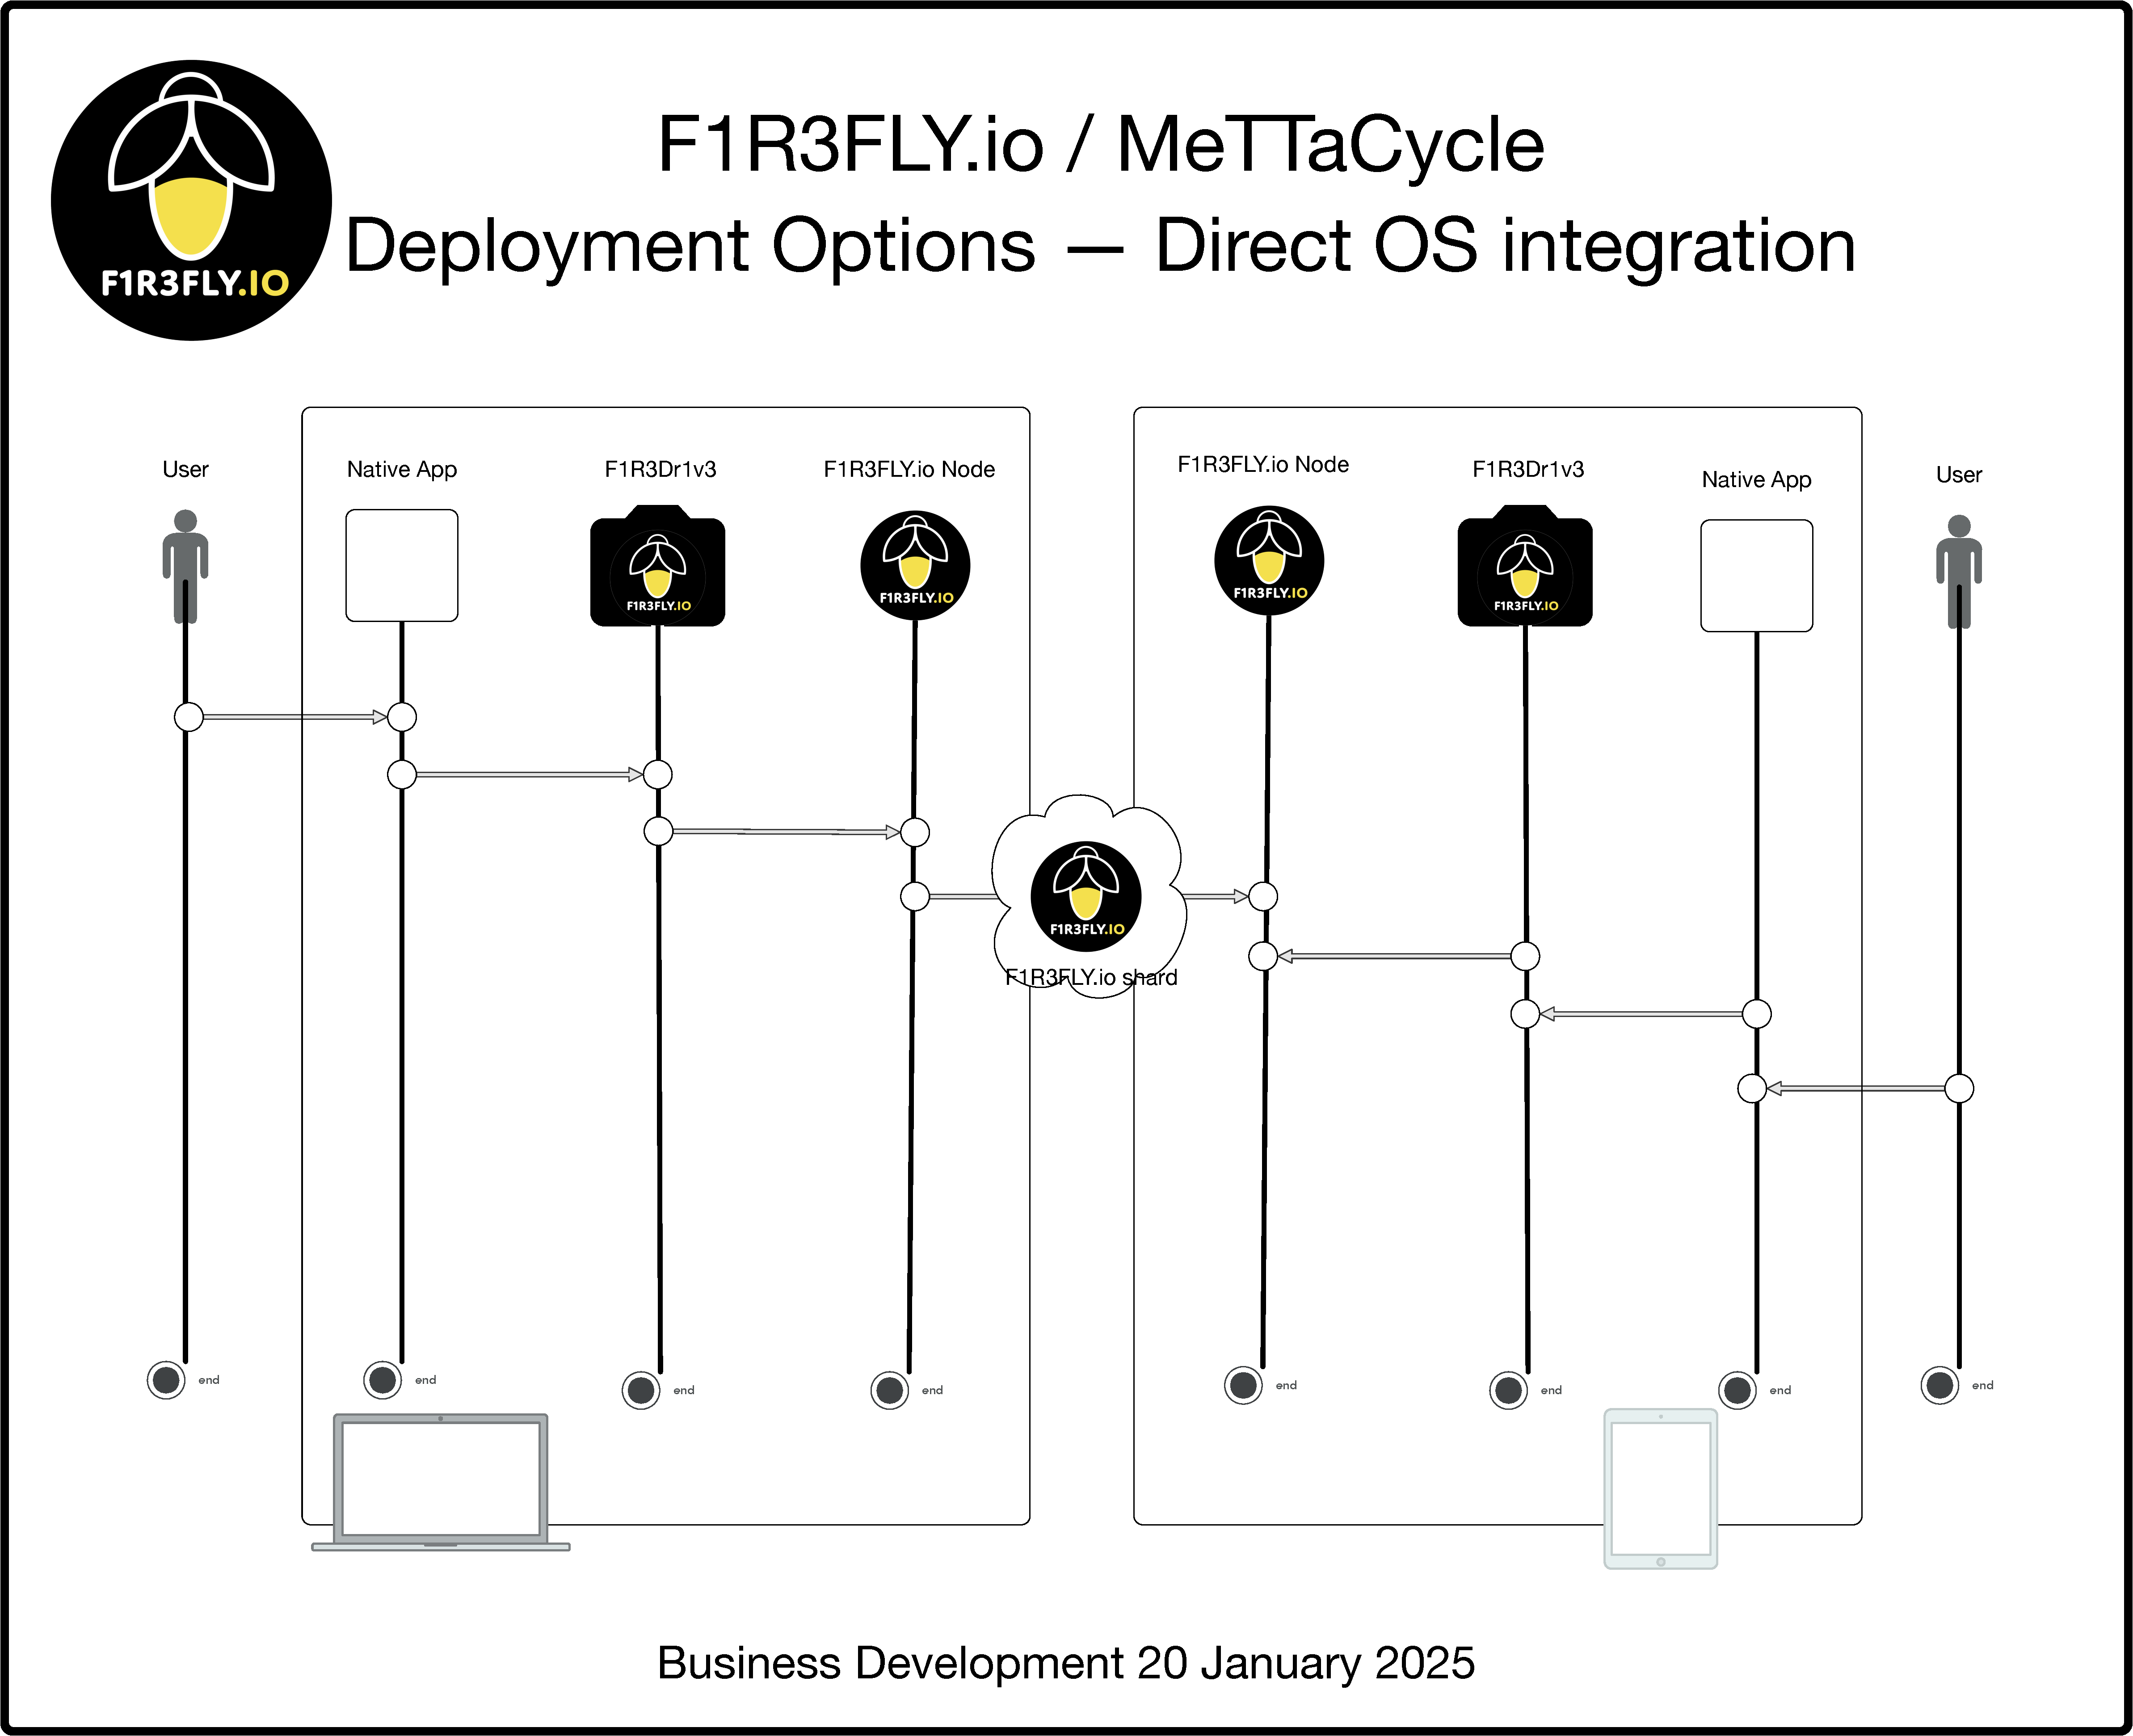
\includegraphics[scale=0.15]{MeTTaCycleArchitecture2025OSDeployment.pdf} \\
  \caption{OS/File system deployment}
  \label{MCArch2025OSDeployment}
\end{figure}

\subsection{Integration with social media}

In the case of integration with social media MeTTaCycle offers two
levels of integration. The first of these is importing and exporting
between local caches. For example, Zulip, BlueSky, and Mastodon all
use Postgres as their local instance storage. MeTTaCycle allows import
and export between their Postgres storage and the shard. Thus,
MeTTaCycle becomes a bus between different instances -- without
modification of the social media application stack.

The second of these is a tighter integration involving modifications
to the social media stack in order to add features made possible by
tokenization of capabilities and the integration of agentic AI.

\begin{figure}
  \centering
  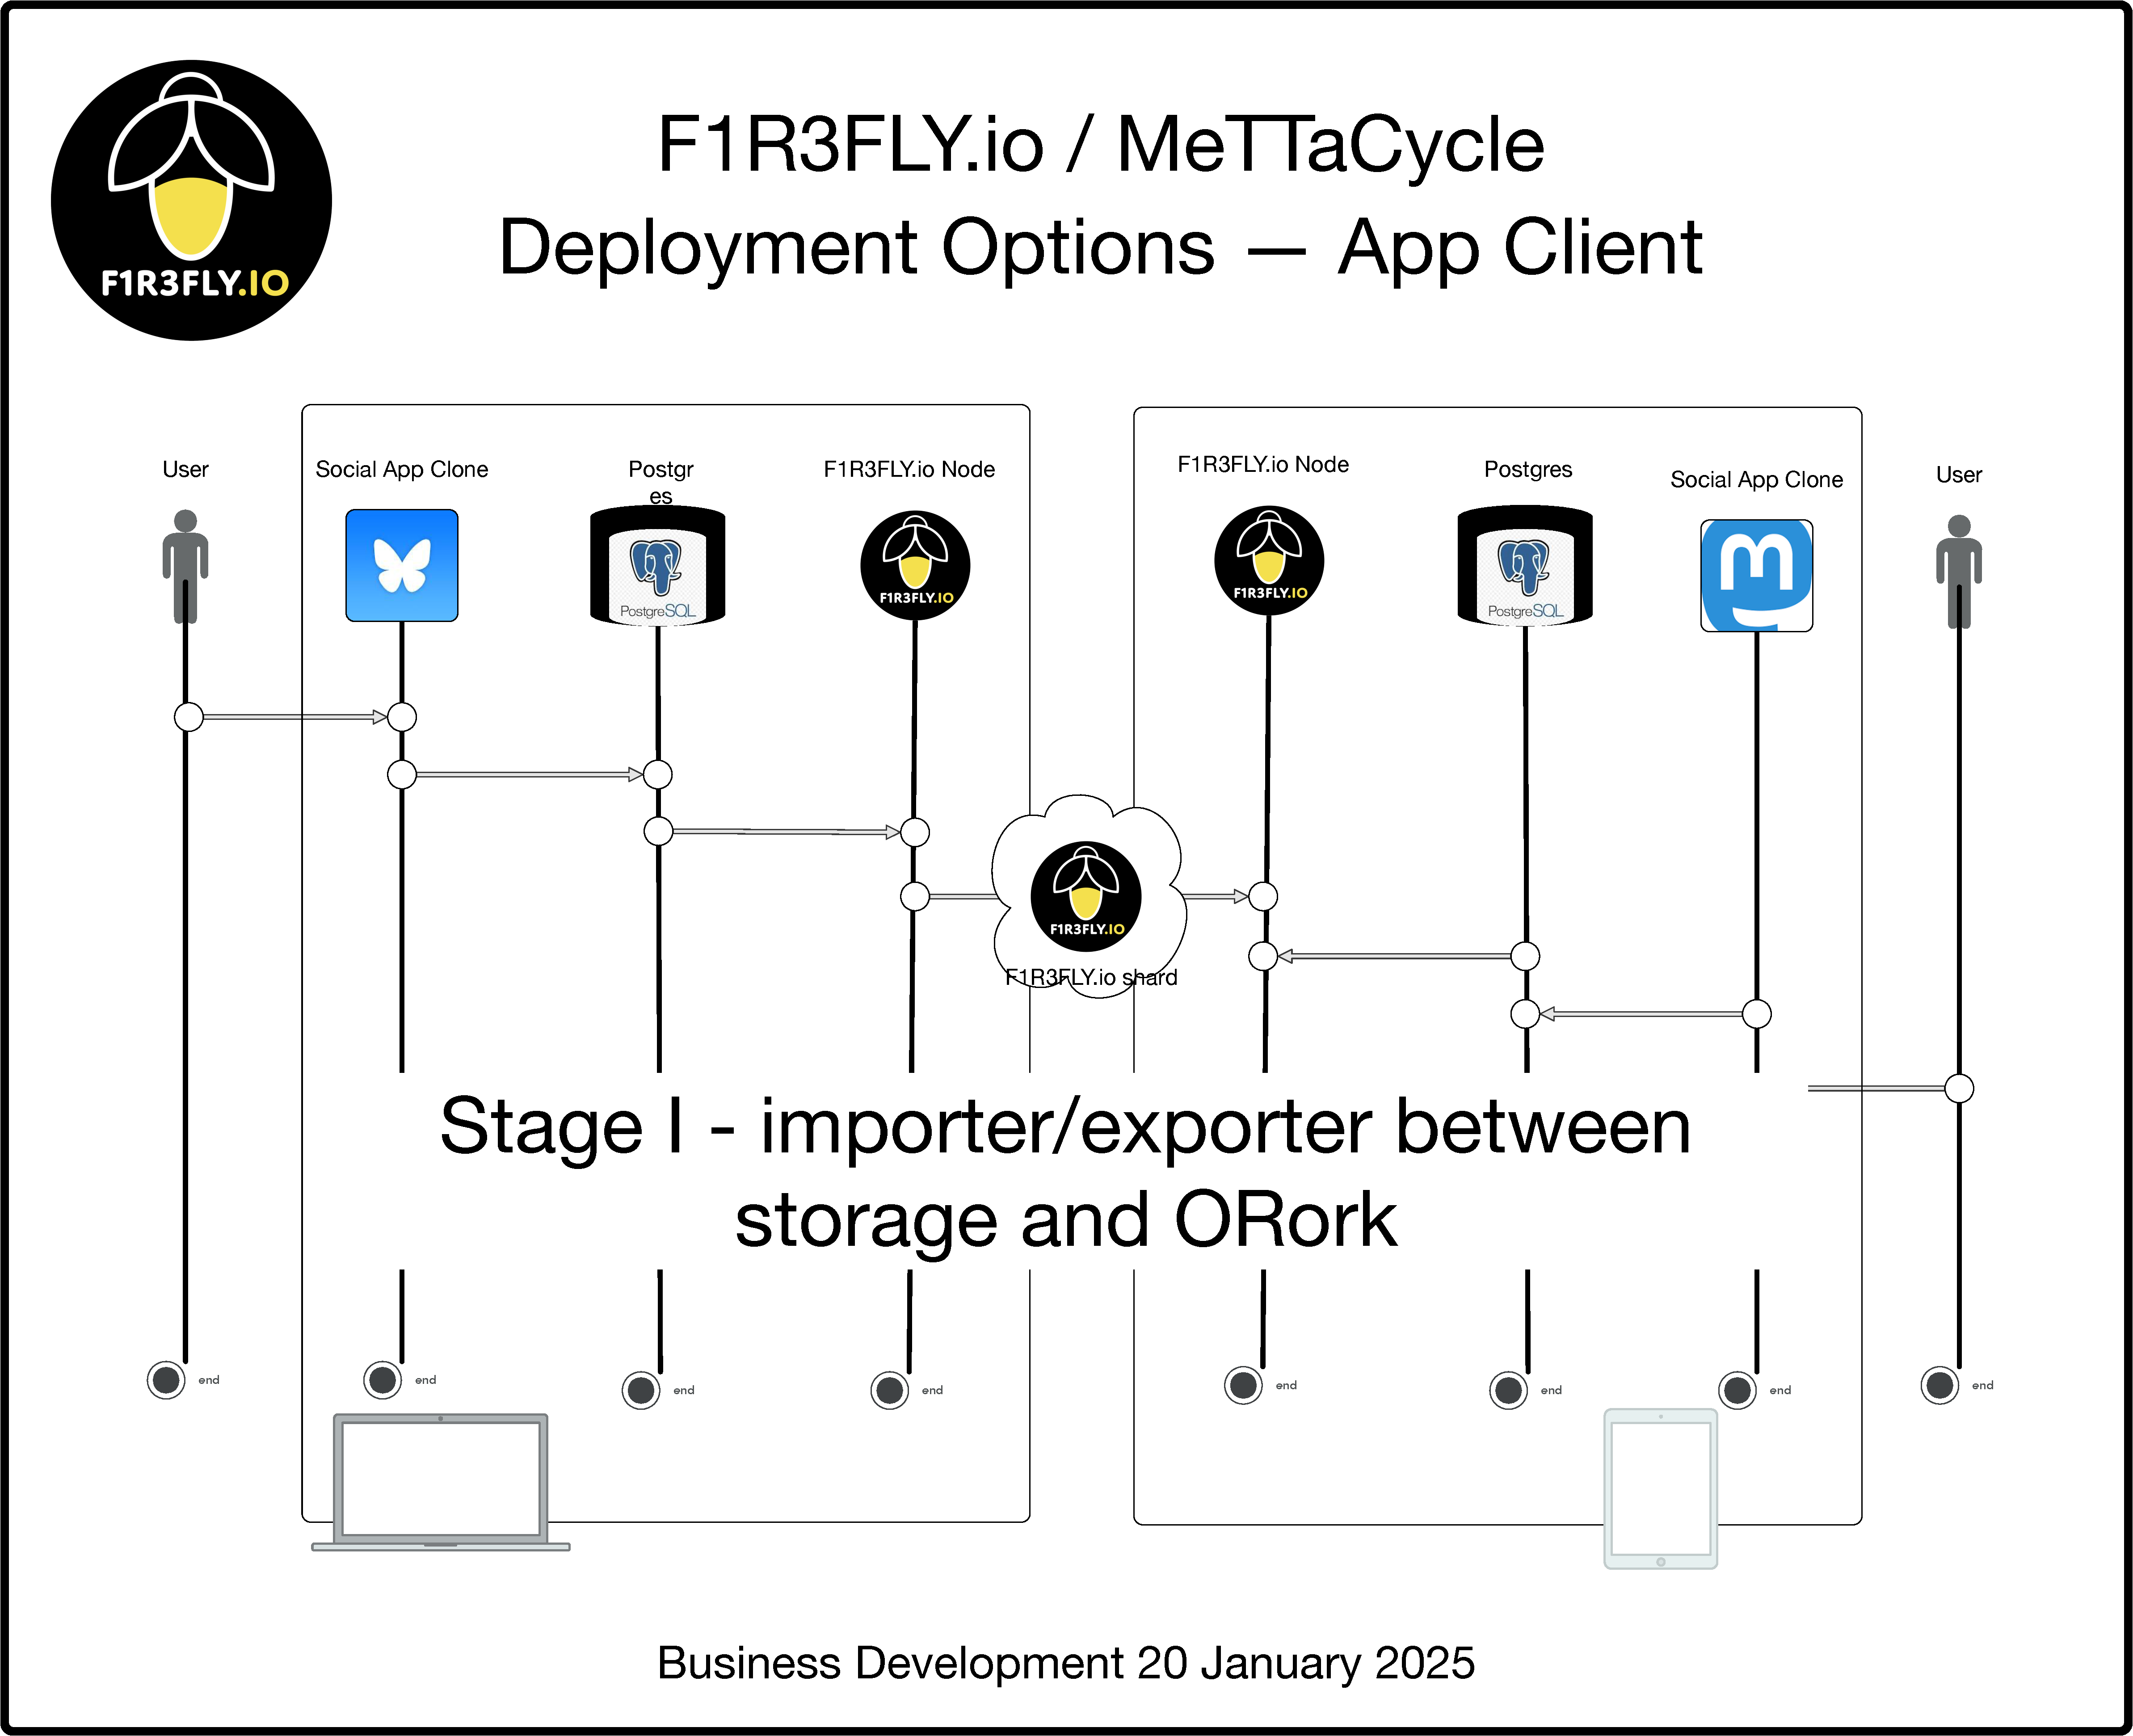
\includegraphics[scale=0.15]{MeTTaCycleArchitecture2025SocialDeployment.pdf} \\
  \caption{Social deployment}
  \label{MCArch2025SocialDeployment}
\end{figure}

\section{Roadmap}

\section{A few use cases}

\subsection{Ocaps for DevOps PaaS}

A particularly compelling application of the $\MC$ architecture lies in the DevOps Platform-as-a-Service (PaaS) sector, where teams seek to configure and monitor projects with minimal overhead. Developers often rely on centralized providers to share infrastructure and capabilities, which can result in vulnerability to deplatforming (for example, when payment providers or credit card companies refuse service) or require complicated permissioning frameworks.

By incorporating object-capabilities (ocaps) into a DevOps environment, $\MC$ could provide a robust mechanism for delegating and attenuating authorization among team members. Specifically, a lightweight plugin or extension built on top of $\MC$ could let organizations share their DevOps resources (such as CI/CD pipelines, artifact repositories, and monitoring dashboards) via secure tokens. This would allow fine-grained access control---even down to the level of revocable, limited-lifespan tokens for specific tasks.

This approach distinguishes itself from existing DevOps PaaS offerings in that it deploys ocaps as the fundamental security model, rather than as an add-on or ad-hoc wrapper. While no current competitor offers a sharing model based on ocaps, the development of such a plugin would likely require its own dedicated team to ensure seamless integration with existing DevOps tools.

An interesting extension of this model would be to empower autonomous AI agents with delegated ocaps for various DevOps operations. For example, an AI-driven build optimizer could be granted a strictly bounded token that allows it to adjust continuous integration parameters without risking broader system access. Such autonomous agents could also facilitate zero-downtime deployments and real-time resource scaling, all while ensuring that their authority remains precisely delimited by the ocaps architecture.

\subsection{Sensors}

A second use case envisions a network of industrial sensors within a smart factory, all powered by $\MC$'s concurrency and transactional semantics. Many factories rely on streams of data from robotic arms, assembly lines, and inventory management systems, feeding downstream analytics to optimize production. A decentralized “marketplace” for sensor data could allow different agents---both human and AI---to connect, filter, and aggregate these streams.

Using $\MC$, sensors and agents become active participants in an economy of data consumption. The architecture’s flexible query language can filter live streams and route relevant information to different processes for anomaly detection or predictive maintenance. The emphasis on concurrency and fine-grained access tokens could enable secure, selective data sharing among industrial partners or even across entire supply chains.

In this environment, autonomous AI agents could automatically negotiate data access or deploy new analytics modules where they detect certain operational inefficiencies. These agents might, for instance, purchase sensor data streams to train local machine-learning models or dynamically grant short-term access credentials to other agents for collaborative filtering. Crucially, the ocaps mechanism ensures they can only access precisely what they are authorized to, preventing them from overstepping their operational bounds.

\subsection{Sandstorm}

Sandstorm has long provided a platform for sandboxed apps that users can self-host, ensuring data ownership. By deploying $\MC$ as an underlying engine for sandstorm deployments, resource owners can store, share, and collaboratively edit data in a decentralized fashion. Attenuation and delegation of capabilities would be governed by tokens: the owner (or a controlling agent) issues tokens to participants, granting privileged or time-limited access to certain documents, files, or worlds. This model aligns with sandstorm.org’s mission of self-hosting and privacy protection, extending it with the added benefits of a censorship-resistant, Byzantine fault tolerant infrastructure.

Because the integration would require modifications or plugin development within the sandstorm stack itself, it might entail a dedicated development effort. The result, however, would unify the user-friendly collaboration tools sandstorm.org is known for with the secure, decentralized capabilities of $\MC$.

AI agents could automate content moderation tasks, track and summarize collaborative work, or even autonomously curate shared documents for improved knowledge management. By granting these agents time-limited tokens to view and potentially modify files, users could safely outsource tasks such as grammar correction, code review, or content organization to intelligent assistants without risking full administrative access over an entire collection.

\subsection{File hosting}

Finally, an obvious and powerful use case for $\MC$ is straightforward file hosting and sharing, akin to Dropbox or Google Drive. Current commercial solutions often rely on crash fault tolerant architectures that scale well but are prone to deplatforming or security breaches at the central provider. There are also open-source alternatives, such as Tahoe-LAFS, that offer strong decentralization and encryption. $\MC$ naturally aligns with the design philosophy behind censorship-resistant file systems, providing concurrency, transactionality, and token-based access.

Leveraging $\FD$'s existing filesystem bridge, a user could simply drag and drop documents into a folder that is mapped onto $\MC$. This approach already offers encryption at rest, with $\FD$'s environment allowing multi-party access via tokenization. The result is a file hosting platform in which censorship is far more difficult, and availability is improved through blockchain-level fault-tolerance. A key question for future work is how to best integrate advanced encryption and chunk-level redundancy strategies (similar to Tahoe-LAFS) into $\FD$'s architecture to further enhance privacy and reliability.

In this file hosting scenario, autonomous AI agents could assist with document indexing, advanced search capabilities, and automated backups. Using token-limited capabilities, agents might be granted read-only access to large sets of stored files, enabling them to provide semantic search or categorization without the risk of unauthorized edits or deletions. This delegation approach would preserve user control while unlocking AI-driven efficiencies in managing and organizing decentralized data.

\section{Conclusion}

Our proposed architecture addresses the defects of the current MeTTa implementation:

\begin{itemize}
    \item GSLTs can specify the semantics of any discrete theory of computation
    \item From a GSLT, we can generate an efficient interpreter for that theory
    \item From a GSLT, we can generate a sound type system customized to that theory
    \item GSLTs allow defining functions inline.
    \item GSLTs let the programmer specify exactly when subexpressions can reduce.
    \item Rather than have a single shared fact database, the facts become part of a query, and the intepreter can produce new fact databases in in response to queries.
    \item Theories can be combined in multiple ways, including concurrent execution.
    \item State updates are transactional.
    \item The automatically generated type systems are provably sound.
    \item When two theories are combined, the system can automatically generate a new type system encompassing both and their interactions.
\end{itemize}


\begin{thebibliography}{99}

\bibitem{Barendregt1991}
Barendregt, Henk (1991). 
``Introduction to generalized type systems.''  
\emph{Journal of Functional Programming}, 1(2): 125--154.

\bibitem{Caires2007}
Caires, Luis (2007). 
``Logical Semantics of Types for Concurrency.'' 
In \emph{Algebra and Coalgebra in Computer Science}, 
Second International Conference, CALCO 2007, Bergen, Norway, August 20--24, 2007, Proceedings.
\url{http://ctp.di.fct.unl.pt/~lcaires/papers/CALCO-Caires-1.0.pdf}

\bibitem{CardelliGordon2000}
Cardelli, Luca, and Andrew D. Gordon (2000). ``Mobile ambients.'' \emph{Theoretical Computer Science}, 240: 177--213.

\bibitem{GoertzelMeredith2024}
Goertzel, Ben, and L. Gregory Meredith. Private communication.

\bibitem{HypercubePaper}
[Placeholder for the Hypercube functor paper reference; “cite the hypercube functor paper”].

\bibitem{kframework}
K Framework.
\url{http://kframework.org}.

\bibitem{Lawvere1963}
Lawvere, William (1963). 
``Functorial Semantics of Algebraic Theories'' (PhD Thesis). 
\url{http://www.tac.mta.ca/tac/reprints/articles/5/tr5abs.html}.

\bibitem{MeredithRadestock2005}
Meredith, L.~Gregory, and Matthias Radestock (2005). 
``A Reflective Higher-order Calculus.'' 
\emph{Electronic Notes in Theoretical Computer Science} 141(5), 49--67, 22 December 2005. 
\url{https://doi.org/10.1016/j.entcs.2005.05.016}

\bibitem{Stiegler2004}
Stiegler, Marc (2004). \emph{A PictureBook of Secure Cooperation}. \url{http://www.erights.org/talks/efun/SecurityPictureBook.pdf}.

\bibitem{Tate2010}
Tate, Ross, Michael Stepp, and Sorin Lerner (2010). 
``Generating Compiler Optimization from Proofs.'' 
In \emph{POPL '10: Proceedings of the 37th annual ACM SIGPLAN-SIGACT Symposium on Principles of Programming Languages}, 
pp.\ 389--402, Madrid, Spain. 
ACM, New York, NY, USA. 
\url{http://www.cs.cornell.edu/~ross/publications/proofgen/}.

\bibitem{Trimble2018}
Trimble, Todd (2018). 
``Multisorted Lawvere Theories,'' on the nLab. 
\url{https://ncatlab.org/toddtrimble/published/multisorted+Lawvere+theories}.

\bibitem{WilliamsStay2021}
Williams, Christian, and Michael Stay (2021). ``Native Type Theory.'' \emph{Proceedings of the Fourth Annual Conference on Applied Category Theory}. EPTCS 372 (2022), 116--132.

\end{thebibliography}
\end{document}
